\chapter{Introduction}
\label{c:intro}

\note{Introductory text goes here!}

This paper introduces a family of algorithms for finding maximum common
substructures in a broad class of objects that includes both graphs and
hypergraphs.

\section{Maximum Common Induced Subgraph}

We begin with a well-known problem: maximum common induced subgraph (MCIS). A
graph $G$ is a pair $(V, E)$, where $V = V(G)$ is the vertex set and $E = E(G)$
is the edge set. Each element of $E$ is a two-element subset of $V$, whose
elements are referred to as its endpoints. For example, we may have $V = \{1,
2, 3, 4, 5\}$ and $E = \{\{1,2\}, \{1,3\}, \{2,3\}, \{3,4\}, \{4,5\}, \{4,6\},
\{5,6\}\}$. This graph may be drawn as shown in Figure A, with a point for each
vertex and a line for each edge.  The positions of the points in the plane have
no significance.

\begin{figure}[h!]
\centering
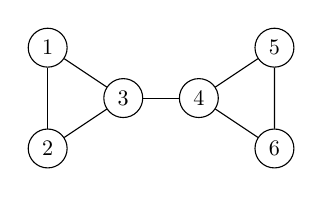
\begin{tikzpicture}[scale=0.8, every node/.style={scale=0.8}]
%\begin{tikzpicture}
  \node [draw,circle] (1) at (0,1.6) {1};
  \node [draw,circle] (2) at (0,0) {2};
  \node [draw,circle] (3) at (1.2,.8) {3};
  \node [draw,circle] (4) at (2.4,.8) {4};
  \node [draw,circle] (5) at (3.6,1.6) {5};
  \node [draw,circle] (6) at (3.6,0) {6};
  \draw (1) -- (2);
  \draw (1) -- (3);
  \draw (2) -- (3);
  \draw (3) -- (4);
  \draw (4) -- (5);
  \draw (4) -- (6);
  \draw (5) -- (6);
\end{tikzpicture}
\caption{Figure A TODO: add caption}
\end{figure}

Two graphs are isomorphic if they can be drawn identically. Thus, the graph in
Figure B is isomorphic to the graph in Figure A, despite having a different
vertex set. Formally, an isomorphism between graphs $G$ and $H$ is a bijection $f$
between the vertex set of $G$ and the vertex set of $H$, such that if we apply $f$ to
the endpoints of each edge of $G$ we obtain the edge set of $H$. If such an $f$
exists, we say that $G$ and $H$ are isomorphic.

\begin{figure}[h!]
\centering
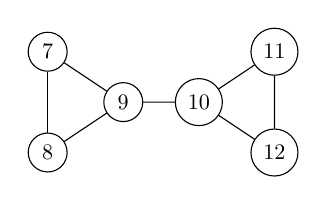
\begin{tikzpicture}[scale=0.8, every node/.style={scale=0.8}]
%\begin{tikzpicture}
  \node [draw,circle] (1) at (0,1.6) {7};
  \node [draw,circle] (2) at (0,0) {8};
  \node [draw,circle] (3) at (1.2,.8) {9};
  \node [draw,circle] (4) at (2.4,.8) {10};
  \node [draw,circle] (5) at (3.6,1.6) {11};
  \node [draw,circle] (6) at (3.6,0) {12};
  \draw (1) -- (2);
  \draw (1) -- (3);
  \draw (2) -- (3);
  \draw (3) -- (4);
  \draw (4) -- (5);
  \draw (4) -- (6);
  \draw (5) -- (6);
\end{tikzpicture}
\caption{Figure B TODO: add caption}
\end{figure}

An induced subgraph of $G = (V, E)$ has a subset $W$ of $V$ as its vertex set, and
$\{\{u, v\} \in E \mid u, v \in W\}$ as its edge set; that is, the subgraph
includes all edges of $G$ both of whose endpoints appear in $W$.  The first graph
in Figure C is thus an induced subgraph of the graph in Figure A, whereas the
second graph is not. We say that the set $W$ induces the subgraph.

\begin{figure}[h!]
\centering
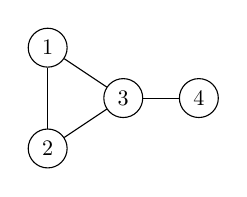
\begin{tikzpicture}[scale=0.8, every node/.style={scale=0.8}]
  \node [draw,circle] (1) at (0,1.6) {1};
  \node [draw,circle] (2) at (0,0) {2};
  \node [draw,circle] (3) at (1.2,.8) {3};
  \node [draw,circle] (4) at (2.4,.8) {4};
  \draw (1) -- (2);
  \draw (1) -- (3);
  \draw (2) -- (3);
  \draw (3) -- (4);
\end{tikzpicture}
\qquad
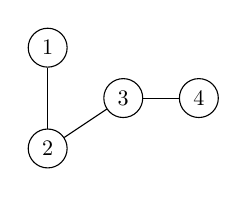
\begin{tikzpicture}[scale=0.8, every node/.style={scale=0.8}]
  \node [draw,circle] (1) at (0,1.6) {1};
  \node [draw,circle] (2) at (0,0) {2};
  \node [draw,circle] (3) at (1.2,.8) {3};
  \node [draw,circle] (4) at (2.4,.8) {4};
  \draw (1) -- (2);
  \draw (2) -- (3);
  \draw (3) -- (4);
\end{tikzpicture}
\caption{Figure C TODO: add caption}
\end{figure}

A \emph{common induced subgraph} of graphs $G$ and $H$ is an induced subgraph of $G$ which
is isomorphic to an induced subgraph of $H$. In figure D, a common induced
subgraph of the two graphs is shown in bold on the first graph, and its
isomorphic subgraph is shown in bold on the second graph.

\begin{figure}[h!]
\centering
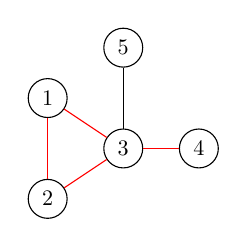
\begin{tikzpicture}[scale=0.8, every node/.style={scale=0.8}]
  \node [draw,circle] (1) at (0,1.6) {1};
  \node [draw,circle] (2) at (0,0) {2};
  \node [draw,circle] (3) at (1.2,.8) {3};
  \node [draw,circle] (4) at (2.4,.8) {4};
  \node [draw,circle] (5) at (1.2,2.4) {5};
  \draw [red] (1) -- (2);
  \draw [red] (1) -- (3);
  \draw [red] (2) -- (3);
  \draw [red] (3) -- (4);
  \draw (3) -- (5);
\end{tikzpicture}
\qquad
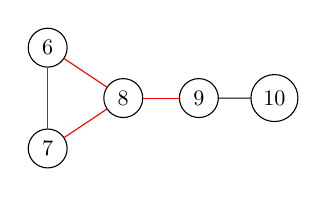
\begin{tikzpicture}[scale=0.8, every node/.style={scale=0.8}]
  \node [draw,circle] (1) at (0,1.6) {6};
  \node [draw,circle] (2) at (0,0) {7};
  \node [draw,circle] (3) at (1.2,.8) {8};
  \node [draw,circle] (4) at (2.4,.8) {9};
  \node [draw,circle] (5) at (3.6,.8) {10};
  \draw [red] (1) -- (2);
  \draw [red] (1) -- (3);
  \draw [red] (2) -- (3);
  \draw [red] (3) -- (4);
  \draw (4) -- (5);
\end{tikzpicture}
\caption{Figure D TODO: add caption}
\end{figure}

A maximum common induced subgraph of $G$ and $H$ is a common induced subgraph of $G$
and $H$ such that no common induced subgraph of the two graphs has a larger
vertex set.

\section{Maximum Common Induced Sub-Hypergraph}

We now describe a problem that includes MCIS as a special case: \emph{maximum common
induced sub-hypergraph (MCISH)} (Cite Bunke et al. 2008). The class of
\emph{hypergraphs} extends the class of graphs by permitting edges containing more
than two vertices. For example, the hypergraph $(\{1,2,3,4,5\}, \{\{1,2,3\}, \{1,4\}\})$
is shown in Figure E; each edge is shown as a shape enclosing two or more
vertices.

%==============================================================================
\section{Thesis Statement}
\label{c:intro:thesisstatement}

This dissertation has the following thesis.

\emph{The structure of the induced subgraph isomorphism and maximum common
subgraph problems allows us to use specialised, compressed data structures to
efficiently represent domains in a backtracking algorithm; by using these
structures we can design algorithms that run faster than the existing state of
the art on many instance classes.}

